\documentclass[journal,12pt,twocolumn]{IEEEtran}
%
\usepackage{setspace}
\usepackage{gensymb}
\usepackage{xcolor}
\usepackage{caption}
%\usepackage{subcaption}
%\doublespacing
\singlespacing

%\usepackage{graphicx}
%\usepackage{amssymb}
%\usepackage{relsize}
\usepackage[cmex10]{amsmath}
\usepackage{mathtools}
%\usepackage{amsthm}
%\interdisplaylinepenalty=2500
%\savesymbol{iint}
%\usepackage{txfonts}
%\restoresymbol{TXF}{iint}
%\usepackage{wasysym}
\usepackage[breaklinks]{hyperref}
\usepackage{amsthm}
\usepackage{amsmath}
\usepackage{mathrsfs}
\usepackage{txfonts}
\usepackage{stfloats}
\usepackage{cite}
\usepackage{cases}
\usepackage{subfig}
%\usepackage{xtab}
\usepackage{longtable}
\usepackage{multirow}
%\usepackage{algorithm}
%\usepackage{algpseudocode}
%\usepackage{enumerate}
\usepackage{enumitem}
\usepackage{mathtools}
%\usepackage{iithtlc}
%\usepackage[framemethod=tikz]{mdframed}
\usepackage{listings}


%\usepackage{stmaryrd}
        \def\inputGnumericTable{}                                 %%

    \usepackage[latin1]{inputenc}                                 %%
    \usepackage{color}                                            %%
    \usepackage{array}                                            %%
    \usepackage{longtable}                                        %%
    \usepackage{calc}                                             %%
    \usepackage{multirow}                                         %%
    \usepackage{hhline}                                           %%
    \usepackage{ifthen}                                           %%
    \usepackage{lscape}                                           %%


%\usepackage{wasysym}
%\newcounter{MYtempeqncnt}
\DeclareMathOperator*{\Res}{Res}
%\renewcommand{\baselinestretch}{2}
\renewcommand\thesection{\arabic{section}}
\renewcommand\thesubsection{\thesection.\arabic{subsection}}
\renewcommand\thesubsubsection{\thesubsection.\arabic{subsubsection}}

\renewcommand\thesectiondis{\arabic{section}}
\renewcommand\thesubsectiondis{\thesectiondis.\arabic{subsection}}
\renewcommand\thesubsubsectiondis{\thesubsectiondis.\arabic{subsubsection}}

%\renewcommand{\labelenumi}{\textbf{\theenumi}}
%\renewcommand{\theenumi}{P.\arabic{enumi}}

% correct bad hyphenation here
\hyphenation{op-tical net-works semi-conduc-tor}

\lstset{
language=Python,
frame=single, 
breaklines=true,
columns=fullflexible
}



\begin{document}
%

\theoremstyle{definition}
\newtheorem{theorem}{Theorem}[section]
\newtheorem{problem}{Problem}
\newtheorem{proposition}{Proposition}[section]
\newtheorem{lemma}{Lemma}[section]
\newtheorem{corollary}[theorem]{Corollary}
\newtheorem{example}{Example}[section]
\newtheorem{definition}{Definition}[section]
%\newtheorem{algorithm}{Algorithm}[section]
%\newtheorem{cor}{Corollary}
\newcommand{\BEQA}{\begin{eqnarray}}
\newcommand{\EEQA}{\end{eqnarray}}
\newcommand{\define}{\stackrel{\triangle}{=}}
\bibliographystyle{IEEEtran}
%\bibliographystyle{ieeetr}
\providecommand{\nCr}[2]{\,^{#1}C_{#2}} % nCr
\providecommand{\nPr}[2]{\,^{#1}P_{#2}} % nPr
\providecommand{\mbf}{\mathbf}
\providecommand{\pr}[1]{\ensuremath{\Pr\left(#1\right)}}
\providecommand{\qfunc}[1]{\ensuremath{Q\left(#1\right)}}
\providecommand{\sbrak}[1]{\ensuremath{{}\left[#1\right]}}
\providecommand{\lsbrak}[1]{\ensuremath{{}\left[#1\right.}}
\providecommand{\rsbrak}[1]{\ensuremath{{}\left.#1\right]}}
\providecommand{\brak}[1]{\ensuremath{\left(#1\right)}}
\providecommand{\lbrak}[1]{\ensuremath{\left(#1\right.}}
\providecommand{\rbrak}[1]{\ensuremath{\left.#1\right)}}
\providecommand{\cbrak}[1]{\ensuremath{\left\{#1\right\}}}
\providecommand{\lcbrak}[1]{\ensuremath{\left\{#1\right.}}
\providecommand{\rcbrak}[1]{\ensuremath{\left.#1\right\}}}
\theoremstyle{remark}
\newtheorem{rem}{Remark}
\newcommand{\sgn}{\mathop{\mathrm{sgn}}}
% \providecommand{\abs}[1]{\left\vert#1\right\vert}
% \providecommand{\res}[1]{\Res\displaylimits_{#1}} 
% \providecommand{\norm}[1]{\lVert#1\rVert}
% \providecommand{\mtx}[1]{\mathbf{#1}}
% \providecommand{\mean}[1]{E\left[ #1 \right]}
% \providecommand{\fourier}{\overset{\mathcal{F}}{ \rightleftharpoons}}
% \providecommand{\ztrans}{\overset{\mathcal{Z}}{ \rightleftharpoons}}
% %\providecommand{\hilbert}{\overset{\mathcal{H}}{ \rightleftharpoons}}
% \providecommand{\system}{\overset{\mathcal{H}}{ \longleftrightarrow}}
% 	%\newcommand{\solution}[2]{\textbf{Solution:}{#1}}
% \newcommand{\solution}{\noindent \textbf{Solution: }}
% \providecommand{\dec}[2]{\ensuremath{\overset{#1}{\underset{#2}{\gtrless}}}}
% \numberwithin{equation}{section}
% %\numberwithin{equation}{subsection}
% %\numberwithin{problem}{subsection}
% %\numberwithin{definition}{subsection}
% \makeatletter
% \@addtoreset{figure}{problem}
\makeatother
\let\StandardTheFigure\thefigure
%\renewcommand{\thefigure}{\theproblem.\arabic{figure}}
\renewcommand{\thefigure}{\theproblem}
\def\putbox#1#2#3{\makebox[0in][l]{\makebox[#1][l]{}\raisebox{\baselineskip}[0in][0in]{\raisebox{#2}[0in][0in]{#3}}}}
     \def\rightbox#1{\makebox[0in][r]{#1}}
     \def\centbox#1{\makebox[0in]{#1}}
     \def\topbox#1{\raisebox{-\baselineskip}[0in][0in]{#1}}
     \def\midbox#1{\raisebox{-0.5\baselineskip}[0in][0in]{#1}}
\vspace{3cm}
\title{ 
	\logo{WiFi Based UGV Operation}
}
\author{Sahukari Chaitanya Varun$^{1}$ \& G V V Sharma$^{2}$ 
%<-this  stops a space
% \thanks{The authors are with the Department
% of Electrical Engineering, Indian Institute of Technology, Hyderabad
% 502285 India .  e-mail: 1. ee19btech11040@iith.ac.in
% 2. gadepall@iith.ac.in}% <-this % stops a space
%%\thanks{J. Doe and J. Doe are with Anonymous University.}% <-this % stops a space
%%\thanks{Manuscript received April 19, 2005; revised January 11, 2007.}}
}
% make the title area
\maketitle
%\newpage
\tableofcontents
\renewcommand{\thefigure}{\theenumi}
\renewcommand{\thetable}{\theenumi}
\bigskip
\begin{abstract}
%
This manual shows how to develop a web controller to operate on UGV
%
\end{abstract}
\section{Building UGV}
%
\begin{enumerate}[label=\thesection.\arabic*
,ref=\thesection.\theenumi]
\item Use the below manual for assembly and to configure the connections of the UGV (ESP32, Motor Driver and Motors).
\begin{lstlisting}
https://github.com/gadepall/EE5161/blob/main/ugv/manual.pdf
\end{lstlisting}
\end{enumerate}
\section{Implementation of the Web Controller}
\begin{enumerate}[label=\thesection.\arabic*
,ref=\thesection.\theenumi]
\item Get the required code from 
\begin{lstlisting}
https://github.com/Chaitanya-Varun/Intro-to-UAV/blob/main/WiFi_UGV_Controller/WiFi_UGV_Controller.ino
\end{lstlisting}
%
\item Now change the SSID and password in the required field in the code corresponding to the local WiFi you use for operation.
\item Compile and Upload the code to ESP32 using a microUSB (or wirelessly) and open the Serial Monitor in Arduino IDE. While uploading the code make sure to press the boot key on the ESP32 to flash the code into memory.
\item Obtain the IP Address of ESP32 and paste it on any web browser. If the IP Address is not visible, press the enable key on ESP32 to rerun the initialization.
\end{enumerate}
\section{Using the Web Controller}
\begin{figure}[h]
    \centering
    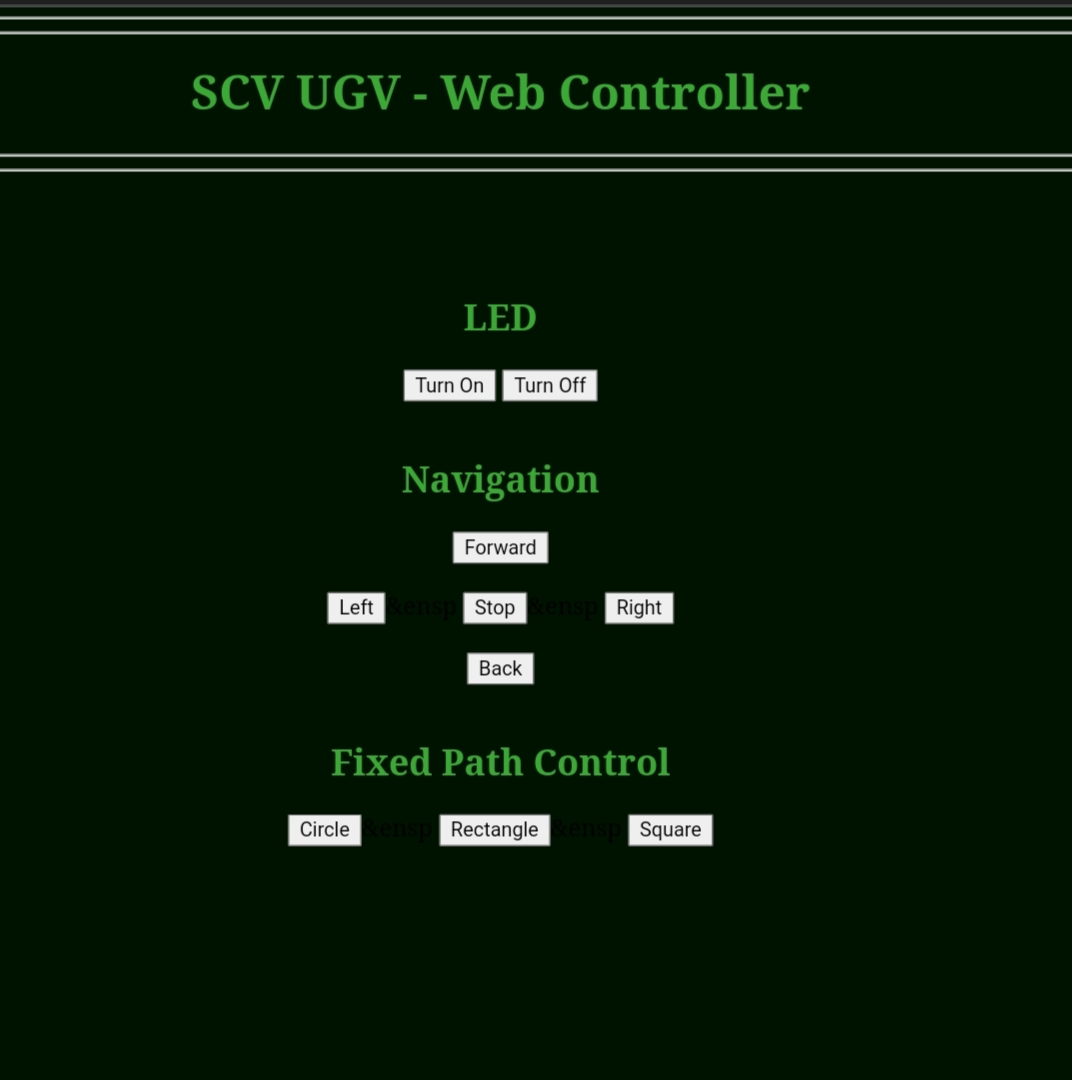
\includegraphics[width=9cm,height=8cm]{figs/web_interface.jpg}
    \caption{User Interface}
    \label{fig:web_interface}
\end{figure}
The web interface would be as shown in the figure \ref{fig:web_interface}. As it runs on a web platform, it can be used on any device (laptop or mobile). The functionalities cover
\begin{itemize}
    \item Turning the LED ON and OFF.
    \item Navigation Commands which include 
    \begin{itemize}
        \item Forward : For making the bot move forward.
        \item Back : For making the bot move backward.
        \item Left : For making the bot move left.
        \item Right : For making the bot move right.
        \item Halt : For making the bot to halt.
    \end{itemize}
    \item Trace fixed paths such as 
    \begin{itemize}
        \item Rectangle
        \item Square
        \item Circle*
    \end{itemize}
\end{itemize}
The web interface is written in basic HTML code directly from the Arduino IDE. When a button is presssed, a corresponding string request will be sent to local WiFi server. The server then broadcasts onto the connected devices, where our ESP32 acts as a client. The received string is decoded to its required functionality. 
\end{document}
